\section{Preliminary Study: Why Active Localization Fails on Outdated Maps}
\label{sec:preliminary}
% ~0,8 pág. Números só por macro (numbers.tex). Fig.~\ref{fig:motivation}.
% (1) Em S2, a PPO não se distingue da reta em sucesso: \vOneSuccessPpoSTwo\% × \vOneSuccessStraightSTwo\%,
%     IC hierárquico da diferença [\vOneDiffSuccessSTwoLow; \vOneDiffSuccessSTwoHigh] p.p.; ~2/3 da distância nos
%     sucessos (\vOneDistSuccessPpoSTwo × \vOneDistSuccessStraightSTwo km); mais localizações falsas
%     (\vOneFalseLocPpoSTwo\% × \vOneFalseLocStraightSTwo\%).
% (2) O sucesso de todos os métodos cai com o índice de mudança (F1); a covariável de cor, independente do
%     descritor, aponta na mesma direção (Spearman de \vOneRhoColorMin a \vOneRhoColorMax, F2).
% (3) Mecanismo M1 (\vOneMOneVerdict): localizações falsas visitam células mais mudadas (+\vOneMOneChangeDiff,
%     IC [\vOneMOneChangeDiffLow; \vOneMOneChangeDiffHigh]), mas não mais distintivas nem mais que as da reta.
%     ATENÇÃO: isso muda a tese do PLANO_ARTIGO.md §1 (ver STATUS_V3.md).
\begin{figure}[t]
\centering
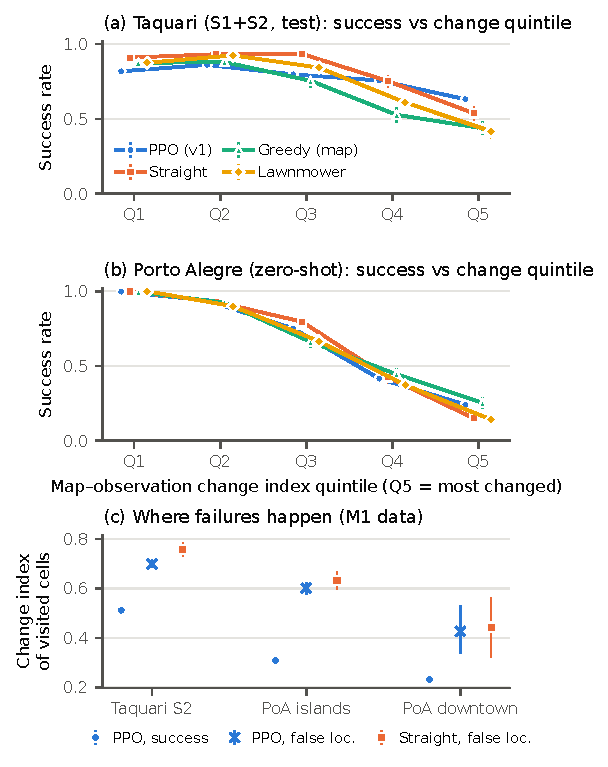
\includegraphics[width=\columnwidth]{figures/fig2_v1_motivation.pdf}
\caption{Preliminary study (v1). (a,b) Success rate by map--observation change-index quintile. (c) Change index of the cells visited in successful and false-localization episodes.}
\label{fig:motivation}
\end{figure}
